\section{Framework}

Zur Umsetzung der Simulation verwenden und erweitern wir das Java Framework \emph{Tortuga}\footnote{\texttt{http://code.google.com/p/tortugades/}}, welches die grundlegenden Funktionalit�ten einer ereignisdiskreten Simulation anbietet. Mit Hilfe aspektorientierter Programmierung wird erm�glicht, dass innerhalb des Programmcodes der selbstdefinierten Entit�tsklassen jederzeit Zugriff auf die Simulation m�glich ist um beispielsweise ein neues Ereignis zu registrieren.\footnote{N�heres zum Thema aspektorientierter Programmierung kann der geneigte Leser zum Beispiel \textcite{kiczales1997aspect} entnehmen. \textcite{laddad2003aspectj} beleuchtet die AspectJ-Erweiterung f�r aspektorientiertes Programmieren in Java genauer.}

Basisklassen f�r eine Simulation und Entit�ten sind in Tortuga vorhanden, wobei die abstrakte Klasse \emph{org.mitre.sim.DefaultEntity} vom Frame\-work\-nutzer erweitert werden muss.

\begin{figure}[t]
	\begin{center}
    	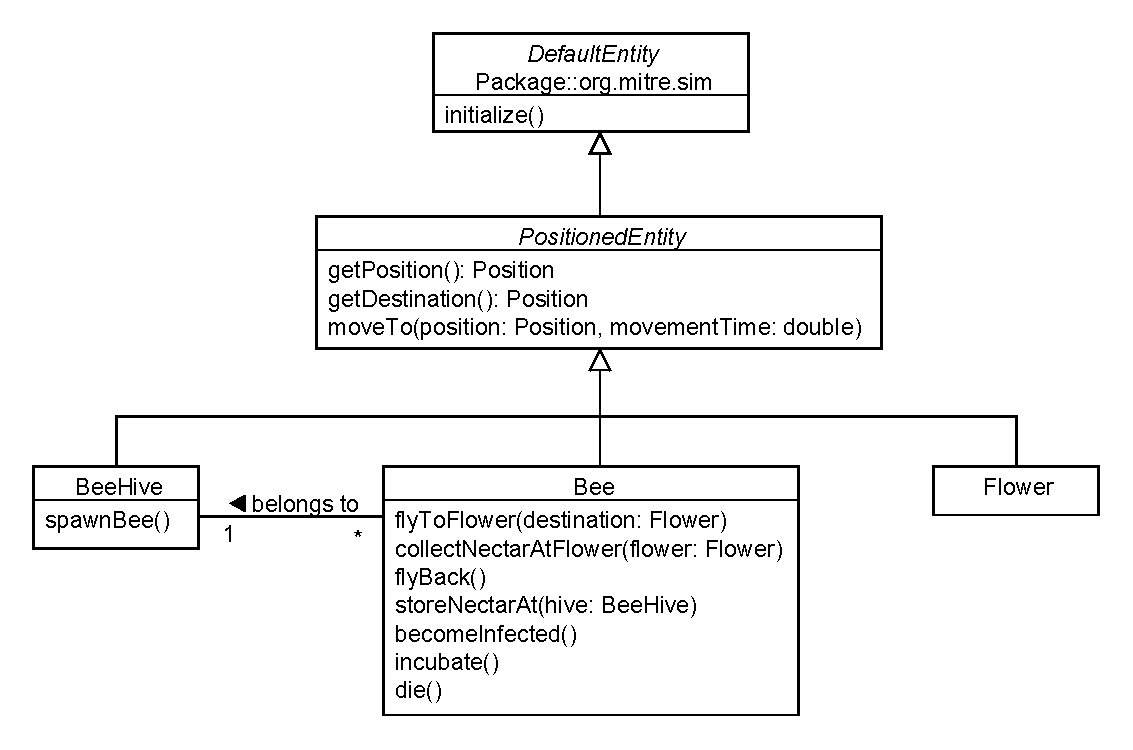
\includegraphics[width=1\linewidth]{entities}
  \caption{UML-Klassendiagramm der Simulationsentit�ten. Private oder nicht simulationsbezogene Methoden und Attribute wurden aus �bersichtlichkeitsgr�nden weggelassen.}
  \label{img:entities} 
	\end{center}
\end{figure}